\documentclass[12pt]{article}

\setlength{\topmargin}{-.75in} \addtolength{\textheight}{2.00in}
\setlength{\oddsidemargin}{.00in} \addtolength{\textwidth}{.75in}

\usepackage{amsmath,color,graphicx,array,multirow,rotating, enumerate}
\usepackage{type1cm}
\usepackage{eso-pic}
\usepackage[hmargin=2cm,vmargin=1.3cm]{geometry}
\usepackage{mathabx}
\usepackage[rflt]{/Users/jgates/desktop/latex/floatflt}
\usepackage[table]{xcolor}
\nofiles

\def\Tab#1{\tabular[t]{>{\rule[-1ex]{0pt}{3ex}}c}#1\endtabular}
\newcolumntype{C}{@{}c@{}}

\pagestyle{empty}
\newcounter{ProbNum}
\setlength{\parindent}{0in}

% Watermark: graph paper
\newcommand\BackgroundPic{
\put(0,0){
\parbox[b][\paperheight]{\paperwidth}{%
\vfill
\centering

\includegraphics[width=\paperwidth,height=\paperheight,keepaspectratio]{/Users/jgates/desktop/latex/pics/plain.pdf}%
\vfill
}}}

%Diagram box command [v space][content]
\newcommand{\diagrambox}[2][40 mm]{
\framebox{\parbox{175 mm}{#2 \hfill \\ \vspace{#1}}}

\bigskip
}

% MakeList: [example number] [content]
\newcommand{\MakeList}[2]{
\begin{enumerate}[#1] \itemsep1pt \parskip0pt \parsep0pt  

#2
\end{enumerate}
}

\begin{document}



{\Large Problems tagged with standards:}CAPM
\bigskip 
% Number 100
% CAPM AMM
% Car speeds up, slows down: rel. easy, pairs with 90
% MIT Physics for Teachers LON-CAPA

% Watermark
\AddToShipoutPicture*{\BackgroundPic}

\addtocounter {ProbNum} {1}

%\begin{floatingfigure}[r]{.3\textwidth}
%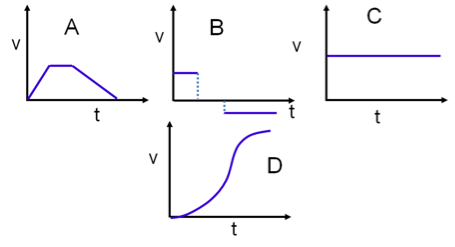
\includegraphics[scale=.4]{/Users/jgates/desktop/latex/pics/vgraph1.png}
%\end{floatingfigure}
 
{\bf \Large{100.}} A car starting from rest speeds up to ${30~\frac{m}{s}}$ with constant acceleration in 15 seconds. Then, it travels at ${30~\frac{m}{s}}$ for 10 seconds. Finally, it brakes to a stop in 30 seconds with constant acceleration. 

 \bigskip

\indent How far does it travel in the 55 second time period?  
 

\bigskip 
\vspace{6mm}% Number 110
% CAPM Motionmap
% Car speeds up, slows down: MC pick motion map
% MIT Physics for Teachers LON-CAPA

% Watermark
\AddToShipoutPicture*{\BackgroundPic}

\addtocounter {ProbNum} {1}

\begin{floatingfigure}[r]{.3\textwidth}
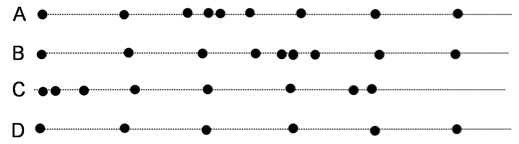
\includegraphics[scale=.4]{/Users/jgates/desktop/latex/pics/Motionmap1.png}
\end{floatingfigure}
 
{\bf \Large{110.}} Driving a car in the positive x direction at a speed of 60 mph, Mary tests her brakes by coming to a complete stop in 4 seconds. Then she accelerates to her original speed of 60 mph in 8 seconds. A motion diagram is created by illuminating her car with a strobe at 2 second intervals. 

 \bigskip

\indent Which of the following best represents the correct diagram? Mary�s car is represented by a dot.   
 

\bigskip 
\vspace{6mm}% Number 20
% UFPM CAPM Friction KFriction 
% Box sliding down frictionless incline: a, motion

% Watermark
\AddToShipoutPicture*{\BackgroundPic}

\addtocounter {ProbNum} {1}

\begin{floatingfigure}[r]{.25\textwidth}

\includegraphics{/Users/jgates/desktop/latex/pics/incline1.png}
\end{floatingfigure} 

{\bf \Large{20.}} A box of mass ${m}$ slides with an initial velocity of ${3~\tfrac{m}{s}}$ down a ramp which is inclined ${20^\circ}$ from the horizontal.  The coefficient of kinetic friction between the ramp and box is .45.

\bigskip

\indent  a. Determine the direction and magnitude of the acceleration of the box as it slides down the incline. 

\bigskip 
b. Discuss the subsequent motion of the box (qualitatively - no numbers are necessary).

\bigskip 
\vspace{6mm}% Number 90
% CAPM GMM
% v graphs - conceptual q
% MIT Physics for Teachers LON-CAPA

% Watermark
\AddToShipoutPicture*{\BackgroundPic}

\addtocounter {ProbNum} {1}

\begin{floatingfigure}[r]{.3\textwidth}
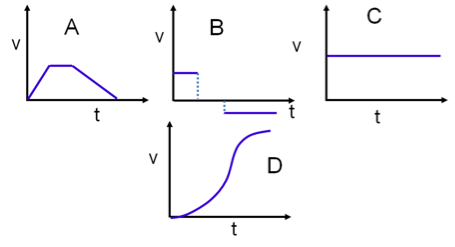
\includegraphics[scale=.4]{/Users/jgates/desktop/latex/pics/vgraph1.png}
\end{floatingfigure}
 
{\bf \Large{90.}} A car starting from rest speeds up to ${30~\frac{m}{s}}$ with constant acceleration in 10 seconds. Then, it travels at ${30~\frac{m}{s}}$ for 10 seconds. Finally, it brakes to a stop in 20 seconds with constant acceleration. 
\bigskip

\indent Which of the following graphs represents the speed of the car versus time?  
 

\bigskip 
\vspace{6mm}\end{document}